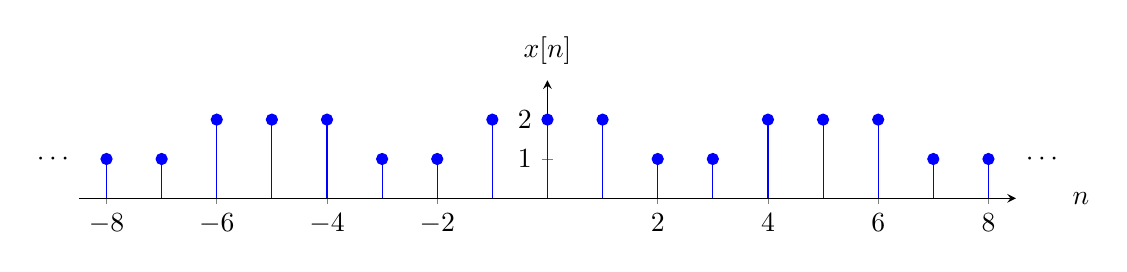
\begin{tikzpicture}[scale=1]	


\begin{filecontents}{example313.dat}
o    xo
-8 1
-7 1
-6 2
-5 2
-4 2
-3 1
-2 1
-1 2
0 2
1 2
2 1
3 1
4 2
5 2
6 2
7 1
8 1
\end{filecontents}

    \begin{axis}[
    		name=axis1,
		y=0.5cm,
		x=0.7cm,
		 clip=false,
		 xmin=-8.5,xmax=8.5,
		 xlabel= $n$,
		 ylabel={$x[n]$},
		 ymin=0,ymax=3,
		 axis lines=middle,
         %xtick={-3.1416, -2.513, -1.885, -1.257, -0.6283, 0, 0.6283, 1.257, 1.885, 2.513, 3.1416, 6.2832},
         %xticklabels={-5, -4, -3, -2, -1, 0, 1, 2, 3, 4, 5, 10 },
		 ytick={1, 2},
		 yticklabels={1,2},
		 every axis x label/.style={at={(ticklabel* cs:1.05)}, anchor=west,},
		every axis y label/.style={at={(ticklabel* cs:1.05)}, anchor=south,},
     ]
		%\addplot [red, smooth, mark=none] table [x={o}, y={xo}] {example313.dat;%
		\addplot [blue, ycomb, mark=*] table [x={o}, y={xo}] {example313.dat};%

		\node at (axis cs:8.5, 1) [anchor=west] { $\cdots$ };
		\node at (axis cs:-8.5, 1) [anchor=east] { $\cdots$ };		
    \end{axis}

%
% %\pause
%     \begin{axis}[
%     	name=axis2,
%         	at={($(axis1.south east)+(0,-0.5cm)$)},anchor=north east,
% 		y=0.25cm,
% 		x=0.8cm,
% 		 clip=false,
% 		 xmin=-3.5,xmax=10,
% 		 xlabel= $k$,
% 		 ylabel={$Na_k$},
% 		 ymin=-1.5,ymax=6,
% 		 axis lines=middle,
%          xtick={-3.1416, -2.513, -1.885, -1.257, -0.6283, 0, 0.6283, 1.257, 1.885, 2.513, 3.1416, 6.2832},
%          xticklabels={-10, -8, -6, -4, -2, 0, 2, 4, 6, 8, 10, 20 },
% 		 %ytick={-1, 1},
% 		 yticklabels=\empty,
% 		 every axis x label/.style={at={(ticklabel* cs:1.05)}, anchor=west,},
% 		every axis y label/.style={at={(ticklabel* cs:1.05)}, anchor=south,},
%      ]
% 		\addplot [red, smooth, mark=none] table [x={o}, y={xo}] {g_dt_fs/figures/dtfs_square_N20.dat};%.
% 		\addplot [blue, ycomb, mark=*] table [x={o}, y={xo}] {g_dt_fs/figures/dtfs_square_stem_N20.dat};%.
%
% 		\node at (axis cs:10, 3) [anchor=east] { $N=20$ };
%     \end{axis}
%
% %\pause
%         \begin{axis}[
%     	name=axis3,
%     	at={($(axis2.south east)+(0,-0.5cm)$)},anchor=north east,
% 		y=0.25cm,
% 		x=0.8cm,
% 		 clip=false,
% 		 xmin=-3.5,xmax=10,
% 		 xlabel= $k$,
% 		 ylabel={$Na_k$},
% 		 ymin=-1.5,ymax=6,
% 		 axis lines=middle,
%          xtick={-3.1416, -2.513, -1.885, -1.257, -0.6283, 0, 0.6283, 1.257, 1.885, 2.513, 3.1416, 6.2832},
%          xticklabels={-20, -16, -12, -8, -4, 0, 4, 8, 12, 16, 20, 40 },
% 		 %ytick={-1, 1},
% 		 yticklabels=\empty,
% 		 every axis x label/.style={at={(ticklabel* cs:1.05)}, anchor=west,},
% 		every axis y label/.style={at={(ticklabel* cs:1.05)}, anchor=south,},
%      ]
% 		\addplot [red, smooth, mark=none] table [x={o}, y={xo}] {g_dt_fs/figures/dtfs_square_N40.dat};
% 		\addplot [blue, ycomb, mark=*] table [x={o}, y={xo}] {g_dt_fs/figures/dtfs_square_stem_N40.dat};
%
% 		\node at (axis cs:10, 3) [anchor=east] { $N=40$ };
%     \end{axis}

\end{tikzpicture} 